\documentclass[12pt]{report}

% This is the Results section
\usepackage[margin=1.0in]{geometry}
\usepackage{graphicx}
\usepackage{textcomp} % Used for the < and > symbols in text mode, among others
\usepackage[superscript,biblabel,sort]{cite}
\usepackage[subrefformat=parens,labelformat=parens]{subfig}
\usepackage{caption}
\usepackage{gensymb}
\usepackage{longtable}
\usepackage{cleveref}

\bibliographystyle{aip}
\begin{document}
\chapter{Results and Discussion\label{results}}
\section{Validation of P and Q Matrices\label{results:PQValid}}
The energy profiles calculated from the P and Q matrices were compared with the copper energy profiles expected from the parameters defined in Bulatov \emph{et al.}'s code to validate the generated P and Q matrices.  Results from this comparison for the \textlangle{}100\textrangle{} set are shown in \Cref{fig:compare100}, with all six subsets shown in \Cref{appfig:compare100,appfig:compare110,appfig:compare111}.  The calculated energies match exactly the predicted values for all but a few points.  Each data set mismatches the expected energy at 1\textdegree{}, and the tilt data sets also see this mismatch at their second to last data point.

\begin{figure}[ht!]
 \centering
 
 \subfloat[]{\label{fig:compare100Twist}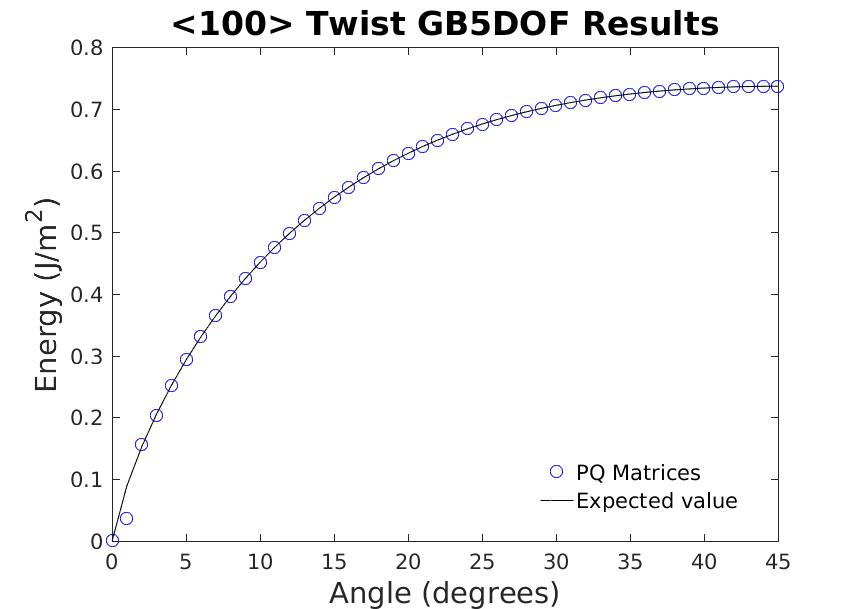
\includegraphics[scale=0.24]{Images/TestPQFit100Twist}}\quad
 \subfloat[]{\label{fig:compare100Tilt}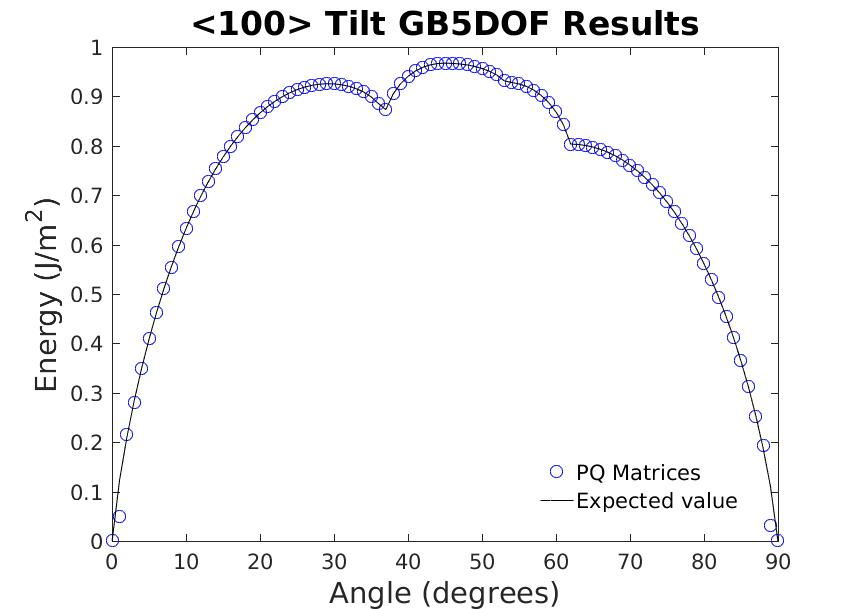
\includegraphics[scale=0.26]{Images/TestPQFit100Tilt}}
 \caption{\label{fig:compare100} The \textlangle{}100\textrangle{} twist \protect\subref{fig:compare100Twist} and tilt \protect\subref{fig:compare100Tilt} results for the P and Q matrices as compared to Bulatov \emph{et al.}'s energy profiles. The expected value was calculated using Bulatov \emph{et al.}'s \lstinline!GB5DOF.m! MATLAB\textsuperscript{\textregistered} script with the default values.  The calculated values were found by inputting the matrices into the \lstinline!GB5DOF.m! script. With the exception of the data points at 1\textdegree{} in both \protect\subref{fig:compare100Twist} and \protect\subref{fig:compare100Tilt} and 89\textdegree{} in \protect\subref{fig:compare100Tilt}, the energies calculated from the matrices matches the expected curves exactly.}
\end{figure}

\section{Fitting Results\label{results:fit}}
Comparisons for the one-dimensional (1D) results from Harbison\cite{harbison2015} and this work are presented in \Cref{fig:100} for the \textlangle{}100\textrangle{} subset.  \Cref{app:graphs} has the full set of comparison graphs shown in \Cref{appfig:100,appfig:110,appfig:111}.  The results show a general decrease in the grain boundary (GB) energies, allowing trends in the different subsets to emerge.  These trends allow for an all around better fit, but there are still some unexpected results present.  The parameters calculated from the fitting procedure are shown in \Cref{table:params} in \Cref{app:params}.

Initial MD recalculations of the \textlangle{}100\textrangle{} symmetric tilt GB energies using the 800 K anneal (\Cref{fig:100Tilt}) showed a deep cusp around 28\textdegree{} which was unexpected.  An analysis of the molecular dynamics (MD) simulation results for this misorientation revealed, in this case, that the two crystals had realigned during the simulation due to abnormally high pressures.  This realignment caused the misorientation angle to change causing the GB energy to be much lower than expected.  Comparison with Harbison's simulation result revealed that the crystal structure from his simulation did not realign.  While Harbison's data was not calculated with the anneal and thus may not represent a global minimum, the data point follows the surrounding data's trend, justifying the use of his result.

Of the symmetric tilt GB energy sets, the \textlangle{}110\textrangle{} set has the most improvement.  All three sets showed a general decrease in the energy, increasing confidence in the accuracy of the fit for GB energies in uranium dioxide (UO\textsubscript{2}).  However, each of these sets provides more opportunity for research.  The \textlangle{}100\textrangle{} set needs more work done for data points after around 50\textdegree{}.  The scatter associated with those points seems to be higher, and the possibility of a slight cusp presents itself around 68\textdegree{}.  It is unknown what behaviors are expected there though because there are so few data points in that region, so additional data would be beneficial.  The \textlangle{}110\textrangle{} set as mentioned shows the most improvement, but there are some low points in the second and third ``humps" not following the trend, indicating further possibility for cusps.  The first part of the function (the first hump) needs additional data to determine the possibility of a cusp between 40\textdegree{} and 50\textdegree{}.  The fitted curve to the \textlangle{}111\textrangle{} set now has an unexpected upward trend.  The scatter associated with these data points is also relatively high, leading to the possibility of a completely different set of functions to define this subset.

The twist GB energy sets vary in their success.  The \textlangle{}100\textrangle{} set shows little difference between Harbison's \cite{harbison2015} work and this work.  There is a slight positive concavity at the end of the fitting for this subset, which is unexpected, indicating the possibility of a cusp.  This cusp may occur around 30\textdegree{}.  The \textlangle{}110\textrangle{} set has a definite decrease in the overall energies, creating a plateau profile.  An additional cusp around 40\textdegree{} is being considered.  The \textlangle{}111\textrangle{} set has the least improvement.  From the Bulatov \emph{et al.}'s work\cite{bulatov2014} this work expected to see a plateau as Harbison's fitting demonstrated.\cite{harbison2015}  Instead, the fitting produced a curved energy profile, indicating the potential for at least one cusp.  A possible location of this cusp is around 35\textdegree{}.  Preliminary work has been done with changing the number of parameters in an effort to maximize the quality of the fit with a minimal number of parameters. \Cref{fig:updatedGraphs} compares the current fitting to the tentative new fitting for three of the six 1D subsets.  These modified fits in general seem to fit better at the cost of additional parameters, with a smaller $\chi_{\textnormal{red}}^2$ value.  Still more parameters may be needed to accommodate additional cusps however.

\Cref{fig:100PQ} shows the comparison between the values calculated from the P and Q matrices and the expected values from the MD calculations for the \textlangle{}100\textrangle{} subset.  All six subsets are shown in \Cref{appfig:100PQ,appfig:110PQ,appfig:111PQ} in \Cref{app:graphs}.  There is an unsolved scaling issue with the \textlangle{}100\textrangle{} tilt subset.  Overall, the results from the P and Q matrices match the fitted values, with a few anomalies needing to be addressed.

\begin{figure}[ht!]
 \centering
 
 \subfloat[]{\label{fig:100Twist}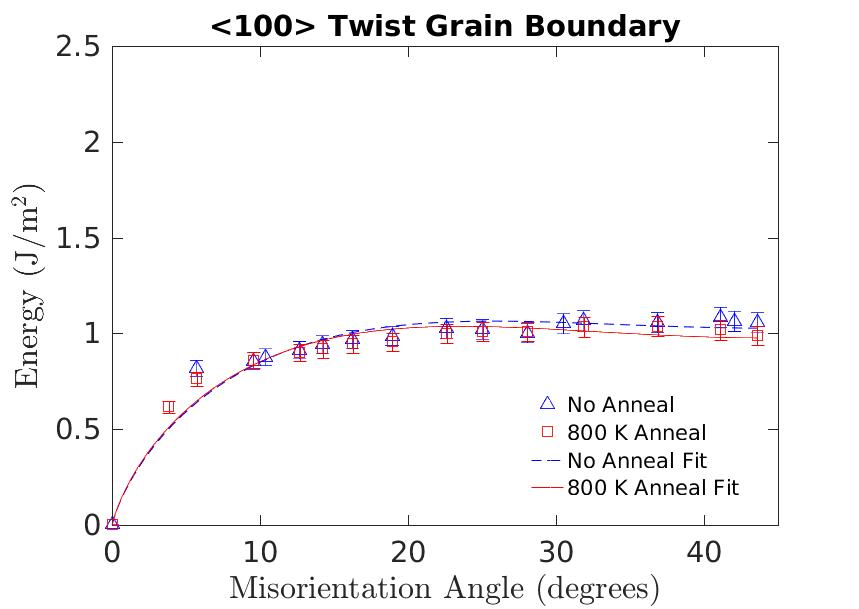
\includegraphics[scale=0.26]{Images/100TwistComparison}}\quad
 \subfloat[]{\label{fig:100Tilt}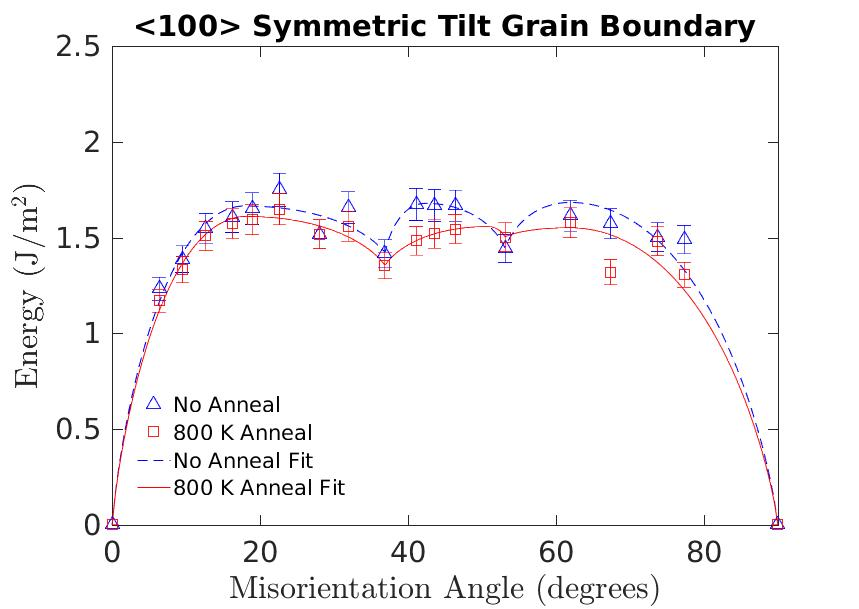
\includegraphics[scale=0.26]{Images/100SymmTiltComparison}}
 \caption{\label{fig:100} The \textlangle{}100\textrangle{} twist \protect\subref{fig:100Twist} and tilt \protect\subref{fig:100Tilt} results.  In general the re-calculated energies are lower, with significant differences around 40\textdegree{} to 50\textdegree{} in the tilt subset.  The positive concavity in the twist subset around 40\textdegree{} is unexpected, and may indicate the presence of a missing cusp.  There is a possible cusp around 30\textdegree{} in the twist subset, and around 68\textdegree{} in the tilt subset. }
 
\end{figure}

\begin{figure}[ht!]
 \centering
 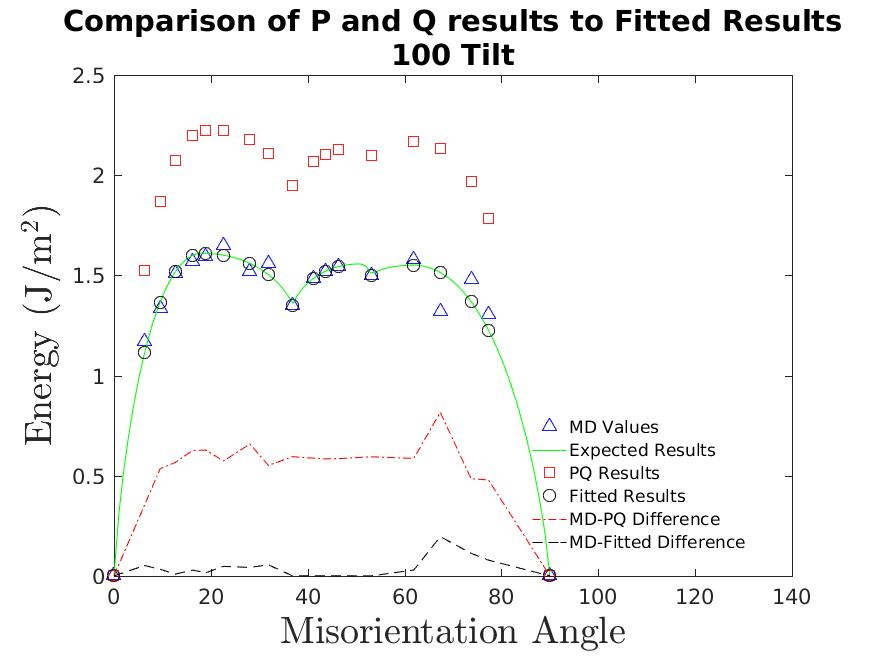
\includegraphics[scale=0.26]{Images/100TiltPQvsMD}
 \caption{\label{fig:100PQ} A comparison of the expected value of the fitted function with the values calculated using the P and Q matrices for the \textlangle{}100\textrangle{} 1D tilt subset.  The MD values are shown for reference.  There is a scaling issue yet to be fixed, but it is uncertain what is causing the scaling issue for this subset.}
\end{figure}

\begin{figure}[ht!]
 
 \begin{minipage}{.5\linewidth}
 \centering
 \subfloat[]{\label{fig:updated100Twist}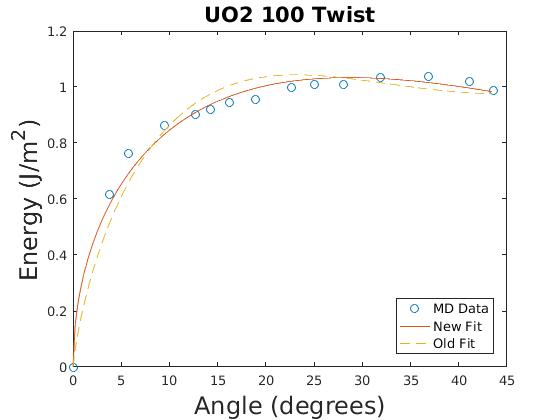
\includegraphics[scale=0.42]{Images/100Twist_marquardt}}
 \end{minipage}%
 \begin{minipage}{.5\linewidth}
 \centering
 \subfloat[]{\label{fig:updated110Twist}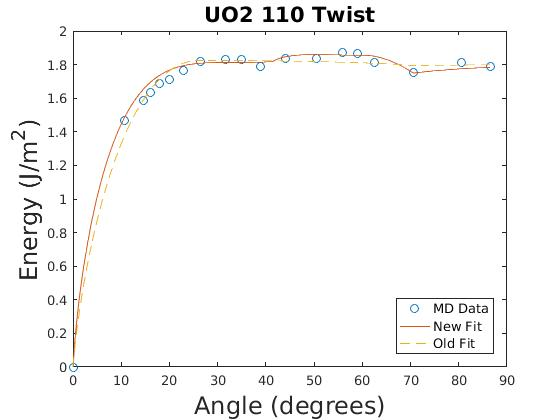
\includegraphics[scale=0.42]{Images/110Twist_vary_shaping_factor}}
 \end{minipage} \par\medskip
 \centering
 \subfloat[]{\label{fig:updated111Twist}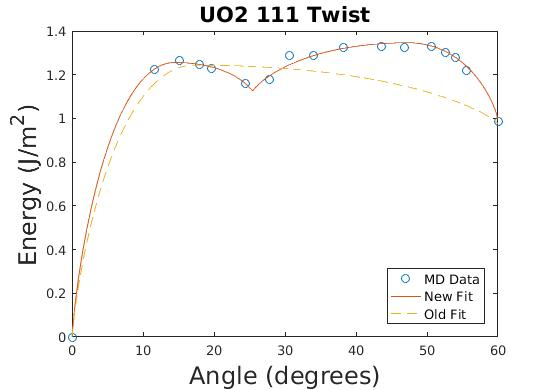
\includegraphics[scale=0.42]{Images/111Twist_marquardt}}
 
 \caption{\label{fig:updatedGraphs} An comparison of current fitting functions with a possible change to the functions.  Original functions are shown as the dashed lines, with the updated functions shown as the solid lines.  MD results are shown for reference. \protect\subref{fig:updated100Twist} shows a possible change from the Read-Shockley-Wolf (RSW) functions to a simple square root function multiplied by an exponential decay.  There is no theoretical basis behind this change however. \protect\subref{fig:updated110Twist} attempts to fit to a cusp around 40\textdegree{}.  Further work can be done to find a better fit for this subset. \protect\subref{fig:updated111Twist} shows the most potential improvement.  The potential fit increases the total number of parameters by three to fit to the cusp around 28\textdegree.  A quick glance at the MD values compared to the fit shows a great improvement from the current fit.}
 
\end{figure}

\section{Reduced Chi-square Results\label{results:chi2red}}
The $\chi_{\textnormal{red}}^2$ values are much smaller than one for every data set regardless of the method used to calculate the statistic, with the exception of the \textlangle{}100\textrangle{} symmetric tilt subset using the P and Q matrices.  This subset has a high $\chi_{\textnormal{red}}^2$ value due to the scaling issue.  Because of the low $\chi_{\textnormal{red}}^2$ values, the fitted functions are known to overfit the data.\cite{bevington2003}  \Cref{table:chi2} lists the $\chi_{\textnormal{red}}^2$ values for the 1D subsets using the two different methods for calculation. \Cref{eq:chi2} shows the equation used to calculate the $\chi^2_{\textnormal{red}}$ value:

\begin{equation}
\label{eq:chi2}
\chi^2_{\textnormal{red}} = \frac{1}{N-n-1} \sum \frac{(\epsilon_{\textnormal{md}} - \epsilon)^2}{e\ \epsilon_{\textnormal{md}}}.
\end{equation}
In this equation, $N$ is the number of observations, $n$ is the number of parameters, $\epsilon_{\textnormal{md}}$ are the energies from MD, $\epsilon$ are the energies from the model, and $e$ is the uncertainty in the MD results.

\begin{table}[ht!]
\centering
\caption{A list of the $\chi_{\textnormal{red}}^2$ results using two different methods: using the P and Q matrices for the various orientations to test the fit, and comparing the results of the 1D fits to the 1D data.  The values for $\chi_{\textnormal{red}}^2$ are all less than one with the exception of the \textlangle{}100\textrangle{} symmetric tilt using the P and Q matrices.  These values indicate an over-fit to the data.}
\label{table:chi2}
\begin{tabular}{{l c c c c}}
1D Subset & \multicolumn{2}{c}{$\chi_{\textnormal{red}}^2$ using P and Q matrices} & \multicolumn{2}{c}{$\chi_{\textnormal{red}}^2$ comparing the 1D fits} \\[5pt]
          & No Anneal & 800 K Anneal & No Anneal & 800 K Anneal \\
\hline
\textlangle{}100\textrangle{} Twist & 0.0953 & 0.1074 & 0.0752 & 0.0722 \\
\textlangle{}110\textrangle{} Twist & 0.1010 & 0.1874 & 0.0400 & 0.0137 \\
\textlangle{}111\textrangle{} Twist & 0.3041 & 0.1139 & 0.4966 & 0.1516 \\
\textlangle{}100\textrangle{} Tilt & 0.1038 & 8.7702 & 0.0846 & 0.0932 \\
\textlangle{}110\textrangle{} Tilt & 4.9799 & 0.3277 & 0.5951 & 0.1762 \\
\textlangle{}111\textrangle{} Tilt & 0.1566 & 0.7814 & 0.1315 & 0.1355 \\
\hline
Overall $\chi_{\textnormal{red}}^2$ & 1.7652 & 1.4893 & 0.2678 & 0.1153 \\
\end{tabular}
\end{table}

\clearpage
\bibliography{gbCharacter}
\begin{longtable}{r l l}
\label{table:params}\\
\caption{This table gives the parameters for UO\textsubscript{2} that generate the energy function.}\\
\hline
\hline
Array number & Parameter name & Parameter value \\
\hline
\endfirsthead
\multicolumn{3}{c}{\tablename\ \thetable\ -- \textit{Continued from previous page}}\\
\hline
Array number & Parameter name & Parameter value \\
\hline
\endhead
\hline
\multicolumn{3}{r}{\textit{Continued on next page.}}\\
\endfoot
\hline
\hline
\endlastfoot
1 & Energy Scaling Factor ($e_{RGB}$) & 1.6012 $J/m^2$ \\
2 & \textlangle{}100\textrangle{} Max Distance & 0.405 \\
3 & \textlangle{}110\textrangle{} Max Distance & 0.739 \\
4 & \textlangle{}111\textrangle{} Max Distance & 0.352 \\
5 & \textlangle{}100\textrangle{} Weight & 50.5 \\
6 & \textlangle{}110\textrangle{} Weight & 4.55 \\
7 & \textlangle{}111\textrangle{} Weight & 0.08 \\
8 & \textlangle{}100\textrangle{} Tilt/Twist Mix Power Law (1) & 0.03325 \\
9 & \textlangle{}100\textrangle{} Tilt/Twist Mix Power Law (2) & 0.00053125 \\
10 & Maximum \textlangle{}100\textrangle{} Twist Energy & 0.60903 \\
11 & \textlangle{}100\textrangle{} Twist Shape Factor & 1.4486 \\
12 & \textlangle{}100\textrangle{} Asymmetric Tilt Interpolation Power & 35.8 \\
13 & \textlangle{}100\textrangle{} Symmetric Tilt First Peak Energy & 1.0058 \\
14 & \textlangle{}100\textrangle{} Symmetric Tilt First $\Sigma5$ Energy & 0.84456 \\
15 & \textlangle{}100\textrangle{} Symmetric Tilt Second Peak Energy & 0.97259 \\
16 & \textlangle{}100\textrangle{} Symmetric Tilt Second $\Sigma5$ Energy & 0.9379 \\
17 & \textlangle{}100\textrangle{} Symmetric Tilt $\Sigma17$ Energy & 0.96881 \\
18 & \textlangle{}100\textrangle{} Symmetric Tilt First Peak Angle & 0.31569 \\
19 & \textlangle{}100\textrangle{} Symmetric Tilt Second Peak Angle & 0.88538 \\
20 & \textlangle{}110\textrangle{} Tilt/Twist Mix Power Law (1) & 3.1573 \\
21 & \textlangle{}110\textrangle{} Tilt/Twist Mix Power Law (2) & 1.9784 \\
22 & \textlangle{}110\textrangle{} Twist Peak Angle & 0.46145 \\
23 & \textlangle{}110\textrangle{} Twist Peak Energy & 1.1444 \\
24 & \textlangle{}110\textrangle{} Twist $\Sigma3$ Energy & 1.0931 \\
25 & \textlangle{}110\textrangle{} Twist 90\textdegree{} Energy & 1.152 \\
26 & \textlangle{}110\textrangle{} Asymmetric Tilt Shape Factor & 3.1843 \\
27 & \textlangle{}110\textrangle{} Symmetric Tilt Third Peak Energy & 1.0514 \\
28 & \textlangle{}110\textrangle{} Symmetric Tilt $\Sigma3$ Energy & 0.61703 \\
29 & \textlangle{}110\textrangle{} Symmetric Tilt Second Peak Energy & 1.0902 \\
30 & \textlangle{}110\textrangle{} Symmetric Tilt $\Sigma11$ Energy & 0.56686 \\
31 & \textlangle{}110\textrangle{} Symmetric Tilt First Peak Energy & 1.1024 \\
32 & \textlangle{}110\textrangle{} Symmetric Tilt Third Peak Angle & 0.88736 \\
33 & \textlangle{}110\textrangle{} Symmetric Tilt Second Peak Angle & 1.8711 \\
34 & \textlangle{}110\textrangle{} Symmetric Tilt First Peak Angle & 2.731 \\
35 & \textlangle{}111\textrangle{} Tilt-Twist Linear Interpolation & 38.201 \\
36 & \textlangle{}111\textrangle{} Twist Shape Factor & 1.2414 \\
37 & \textlangle{}111\textrangle{} Twist Peak Angle & 0.49979 \\
38 & \textlangle{}111\textrangle{} Twist Peak Energy & 0.7971 \\
39 & \textlangle{}111\textrangle{} Symmetric Tilt Peak Angle & 0.25966 \\
40 & \textlangle{}111\textrangle{} Symmetric Tilt Max Energy & 1.0288 \\
41 & \textlangle{}111\textrangle{} Symmetric Tilt $\Sigma3$ Energy & 1.1311 \\
42 & \textlangle{}111\textrangle{} Asymmetric Tilt Symmetry Point Energy & 3.7674 \\
43 & \textlangle{}111\textrangle{} Asymmetric Tilt Scale Factor & 0.053417 \\
\end{longtable}
\end{document}
